\chapter{Deep Reinforcement Learning for Traffic Signal Control along Arterials}
\label{chap:arterial}
% !TEX root = main.tex

% !TEX root = main.tex
\section{Overview}
\label{sec:intro}
Traffic congestion continues to plague urban environments. Traffic signals serve as one of the most critical bottlenecks that cause congestion, but properly timing signals can often effectively mitigate congestion. Many studies proposed methods to optimize signal timings at isolated intersections. These studies range from manually adjusting signal timings based on expected traffic patterns over some time period~\cite{Mill63}, to actuated signals that adjust signal timings around pre-set values based on current traffic patterns~\cite{CoGD13}, and lastly to adaptive signals that more flexibly adjust signal timings to optimize some objective (usually minimize travel time or queue lengths at the intersection). More recently, reinforcement learning (RL) techniques have been applied to the real-time traffic signal control problem for a single intersection~\cite{VaOl16,wei2018intellilight}; these efforts have shown that RL might provide superior performance over conventional methods. 

However, in urban environments, signals are often in close proximity and this complicates the signal timing problem. Specifically, vehicles departing from one signal influence the arrival pattern of vehicles to the next downstream intersection. Thus, optimizing of signal timings for adjacent traffic signals must be done jointly, which is commonly known as coordinating signal timings. Failure to do so can lead to decisions being made at one signal that can deteriorate traffic operations at another. This is similar to the prisoner's dilemma~\cite{poundstone1993prisoner} in game theory in which locally optimal decisions lead to deterioration of global performance. 

Much effort has been performed to design strategies that explicitly consider coordination between adjacent signals. This includes manually adjust offsets (i.e., time between green signal initiation at adjacent intersections)~\cite{urbanik2015signal}, coordinated graphs for information sharing between intersections~\cite{KWBV08,VaOl16}, or simply using a single, central agent to control all the intersections simultaneously~\cite{brockfeld2001optimizing}. However, explicitly coordinating in this way offers many drawbacks. Current coordinated control requires prior knowledge of traffic patterns and road length to calculate optimal offsets, road structure information to build coordinated graph, etc. The obtained solutions are specifi c to the road network structure. When these features change (e.g., when new intersections are considered), the prevailing coordination policy must be created again. Centralized approaches can alleviate this but these result in large-scale optimization problems that are often not computationally feasible, especially in real-time. Information sharing approaches also rely on large communications networks to share information between signals, and such information is not feasible to obtain. Thus, a central question becomes: \textit{can traffic signal controls operating locally with limited information sharing be able to properly coordinate operations on arterials?}

The chapter proposes a method that implicitly provides coordination through a decentralized RL approach. One of the most emphasized point against implicit-coordination is that control will lead to local optimum without explicit coordination. However, this is only true when traffic signals cannot exchange any information between them, like players engaging in a non-cooperative game. If the information can be shared, even it is between adjacent traffic signals only, it is still possible to achieve promising performance with limited communication.

However, such an attempt is non-trivial with respect to the design of rewards and states in RL. While one of the most important measure in transportation area is the average travel time of all vehicles which is hard to measure instantly, existing studies~\cite{Wier00,VaOl16,wei2018intellilight} take an ad-hoc approach to define reward and state for traffic signal control. Usually they define the reward function as a weighted linear combination of several components, such as queue length, waiting time, number of switches in traffic signal, and sum of delay. Their states include components such as queue length, number of cars, waiting time, and current traffic signal. In recent work~\cite{VaOl16,wei2018intellilight}, images of vehicles' positions on the roads are also considered in the state. 

These ad-hoc design will cause several problems that hinder the application of RL in the real world. First, the engineering details in formulating the reward and state could significantly affect the results. For example, if the reward is defined as a weighted linear combination of several terms, the weights on each terms are tricky to set and the minor difference in weight setting could lead to dramatically different results and policies. Second, the state representation could be in a high-dimensional space, especially when using traffic images as part of the state representation~\cite{VaOl16,wei2018intellilight}. Such a high-dimensional state representation will need much more training data samples to learn and the model may not even converge.

In this chapter, we propose a specific reward and state design that is provably suitable for optimizing the average travel time of all vehicles. Specifically, inspired by a classical transportation method~\cite{MP13}, we use the ``pressure'' as reward and the phase and distribution of vehicles as state. We carefully examine this method under an arterial setting with common signal control strategies that were noted in the transportation field~\cite{newell1981blocking}. Specifically, we compare our method with the optimal coordination strategy obtained from the transportation field, which provides a green wave in which vehicles do not have to stop while traversing the arterial. Under the synthetic data where providing a green wave is the optimal solution, the proposed method can achieve the same performance and automatically form a green wave, which proves our effectiveness in achieving coordination. \textit{This is the first time that a RL method in multi-intersection control is interpreted in connection with traditional methods in transportation area.} In summary, our contributions are as follows:
\begin{itemize}
\item We propose that without explicit coordination strategy, RL method through proper reward and state design can also achieve the effect of coordination along the arterial. 
\item We interpret our RL policy in connection with traditional transportation methods. Our model is tested under a well-designed experiment setting on synthetic data, where there is a closed form optimal solution that has been mathematically justified by transportation theories. To the best of our knowledge, this is the first time that the policy learned by RL is corresponded with the cooperation strategy of traditional transportation methods.
\item Our approach is tested on both synthetic and real-world data and the results show that our method achieves the same optimal performance under simplified settings on synthetic data and outperforms various baseline methods in real-world data.
\end{itemize}

\nop{
\begin{figure}[htbp!]
  \centering
   \includegraphics[width=0.48\textwidth]{figures/intro.png}
    \caption{Simultaneous signal setting  determination and coordination}
   \label{fig:intro}
   \vspace{-5mm}
\end{figure}


Conventional coordination consider explicit coordination through analytical optimization under simplified assumption, which cannot be dynamically adjusted to real-time traffic. In recent years, reinforcement learning (RL) techniques have been used on real-time traffic signal control for a single intersection and shown superior performance over conventional methods. Meanwhile, much effort has been performed to design strategies that explicitly coordinate between intersections, such as hand-crafted offsets of phases between intersections, coordinated graphs for information sharing between intersections, or just using one central agent to control all the intersections. However, it is still an open question in the city-wide traffic light control: \textit{to explicitly coordinate, or not?}


Traffic signals are inherently connected:  departures from one intersection directly impact arrival patterns to the next. This leads to strategies that explicitly account for this coordination since adjusting one signal's timings will influence operations at others. Without explicit coordination between individual-level signals, a traffic signal can only optimize based on its own traffic conditions, which can easily lead to deterioration of traffic at other intersections. This is similar to the prisoner's dilemma in game theory. Individual agents move towards optimal solutions locally, but this does not yield a global optimal solution.

However, explicitly accounting for coordination is not computationally efficient. In fact, at the network-wide level, such problems are impossible to formulate and solve in a realistic manner when interactions among a large number of intersection are considered simultaneously. The current coordinated control requires prior knowledge (e.g., have to know traffic pattern and road length to calculate offset, road structure information to build coordinated graph, etc.) and proposes signal control plans for the specified road structure. With new intersections added into the system, the current coordinated control policy may need to be re-organized or re-learned from scratch. Local optimization is more computationally efficient than explicitly coordinated control since it only need to maintain local information.


The chapter stands in the line of non-explicit coordination for the signal control on the arterials. One of the most emphasized points in explicit-coordination is that control will lead to local optimum without explicit coordination. However, this is only true when traffic signals cannot exchange any information between them, like players engaging in a non-cooperative game. If information can be shared between traffic signals, it is still possible to achieve promising performance with limited communication.

However, such an attempt is non-trivial with following questions: a) for an individual intersection, what information of its neighbors needs to be shared to ensure a timely coordination? b) for multiple intersections, how can they learn to optimize the performance of the system as soon as possible to avoid spreading congestions?
To address the first question, in this chapter, we propose to use deep reinforcement learning (DRL) techniques for individual-level control, given the distribution of the vehicle on the approaching and receiving lanes as contextual information from neighboring intersections.
For the second question, learned knowledge from source intersection are transferred to a new one. With each intersection control considered as a subproblem in the larger arterial, we can then re-use the source’s knowledge (e.g., Q-function in RL) for each subproblem in the target, rather than learning from scratch for target intersections.

}


% !TEX root = main.tex

\section{Related Work}
\subsection{Individual traffic signal control.}
Individual traffic signal control has been investigated extensively in the field of transportation. These methods try to optimize the travel time or delay of vehicles~\cite{Gart83,Henr84,Boil06,SeHe97}, building on the assumption that vehicles are arriving and moving in a specific pattern. Recently, reinforcement learning based methods attempt to address this problem by directly learning from the data~\cite{Wier00,MaDH16}. Earlier work using tabular Q-learning~\cite{APK03,ElAb10} can only deal with discrete state representations. Recent work using deep Q-learning~\cite{liLW16,VaOl16,wei2018intellilight} and policy gradient~\cite{MSCH17} can cope with more complex continuous state representation, and hence have shown better performance.

\subsection{Conventional coordinated traffic signal control.}
Conventional coordinated control usually requires the intersections to have the same cycle length, and traffic of selected movements is facilitated through modifying the offset (i.e., the time interval between the beginnings of green lights) between consecutive intersections. In grid networks with homogeneous blocks, like in dense downtown areas, the coordination can be achieved by setting a fixed offset among all intersections~\cite{urbanik2015signal}. However, few networks are so uniform for such simple treatments. In fact, it is not an easy task to even provide coordination along an arterial, given traffic of opposite directions usually cannot be facilitated simultaneously. To solve this problem, some optimization-based methods, such as TRANSYT~\cite{robertson1969transyt} and MAXBAND~\cite{little1981maxband}, are developed to minimize vehicle travel time and/or number of stops at multiple intersections. 
Some traffic control systems such as SCATS and SCOOT also have internal selection or optimization processes to modify cycle length, phase splits and offsets ~\cite{kergaye2010comparative}. However, such approaches still rely on assumptions to simplify the traffic condition, and do not guarantee optimal results in real world.

\subsection{RL-based coordinated traffic signal control.}
Since recent advances in RL  improve the performance on isolated traffic signal control~\cite{VaOl16,wei2018intellilight}, efforts have been performed to design strategies that cooperate multiple RL agents. \cite{KWBV08} and \cite{VaOl16} consider explicit coordination mechanisms between learning agents using coordination graphs, extending \cite{Wier00} using max-plus algorithm. \cite{yang2005intelligent} and~\cite{france2003multiagent} propose to use hierarchical multi-agent RL for global optimization on traffic signal control. Since all the above methods need to negotiate between the agents in the whole network,  they are computationally expensive. 

There are also a line of studies that use individual RL agents to control the traffic signals in the multi-intersection system~\cite{ElAA13,ALUK10,da2006adaptive}. These methods are more scalable, since each agent makes its own decision based on the information from itself and neighboring intersections without explicit coordination. Our proposed method also follows this direction. However, none of existing studies draw a connection with traditional transportation methods. We are the first work to draw such a connection and show that our RL method can automatically learn a green wave policy.

%they only focus on rewards and overlook the adaptability of the algorithms to the real traffic. Therefore, they cannot interpret why the learned light signal changes corresponding to the traffic. In this chapter, we try to test the algorithms in different traffic setting, and add more interpretation other than just reward.

\nop{
Conventional control methods in isolated intersections use closed-form solutions given by optimization of operational parameters based on assumptions and constraints, while reinforcement learning methods have proven useful in this problem as they are able to learn from data collected from sensors in a more intelligent and adaptive way. \Todo-Guanjie, make it shorter


\begin{itemize}
\item Coordinated method
\item non-Coordinated method
\item centralized control(searching space)
\end{itemize}

Isolated traffic signal control has been investigated extensively in the field of transportation. These methods try to optimize the travel time or delay of vehicles~\cite{Gart83,Henr84,Boil06,SeHe97}, building on the assumption that vehicles are arriving and moving in a specific pattern. Recently, reinforcement learning based methods attempt to attack this problem by directly learning from the data~\cite{wiering2000multi,mannion2016experimental}. Earlier work using tabular Q-learning~\cite{APK03,ElAb10} can only deal with discrete state representations. Recent work using deep Q-learning~\cite{li2016traffic,van2016coordinated,wei2018intellilight} and policy gradient~\cite{mousavi_traffic_2017,mousavi_traffic_2017} can cope with more complex continuous state representation, and hence have shown better performance.

However, major challenges lie in the control of multi-intersection scenario, i.e., along an arterial and inside a network. Current methods generally have two categories, centralized methods, and decentralized methods~\cite{SQAS15}. 


Centralized methods are implemented either with pre-defined or with traffic-responsive methods, while both of them are not easy to scale.  Pre-defined centralized approaches usually use historical data to calculate splits and cycle times so as to maximize the flow in a specific direction. One of the widely-used pre-defined centralized coordinated methods in transportation engineering is through "Green Wave", i.e., vehicle will see a progressive cascade of green lights, to optimize the travel time of vehicles along an arterial. The problem with fixed coordination is that the solution is based on an aggregated average traffic pattern, and therefore does not necessarily address real-time situations satisfactorily. Traffic responsive centralized systems, on the other hand, use a centralized agent to control all intersections for the sake of coordination. Each intersection is typically controlled by traffic-responsive methods for changing signal phases. For systems like SCATS or SCOOT, the decisions are made after internal selection and optimization inside the control systems, which may not reflect real-world consequences. \todo{ZY will work on this part}Centralized methods work well only with well-defined traffic volume patterns. In cities where these patterns are not clearly separable (e.g., cities where business centers are no longer located exclusively downtown), coordination may not be effective. What's more, when adding new intersections into the system, centralized methods are not easy to scale, since it may require a large number of central updates of control strategies, or even learning from scratch. 

\nop{Isolated traffic responsive systems, on the other hand, use inductive loop sensors to determine if there is a long queue of stopped cars, but this decision is only locally optimal.
\todo{In both SCATS and SCOOT systems there are coordination between intersections. Maybe say "the decisions are made after internal selection and optimization inside the control systems, which may not reflect real-world consequences"}

In this sense, traffic responsive coordinated control may have a better performance. One type of solution is centralized methods which requires a centralized agent to control all intersections for the sake of coordination. Each intersection is typically controlled by fixed-time plans for changing signal phases, which is largely reply \todo{dependent?} on prior knowledge. For systems like SCATS or SCOOT, the baseline plans of signal settings are predetermined based on engineering experience. This approach works well only in traffic networks with well defined traffic volume patterns\todo{these adaptive methods  do address changes in traffic}. In cities where these patterns are not clearly separable (e.g., cities where business centers are no longer located exclusively downtown), coordination may not be effective. What's more, when adding new intersections into the system, centralized methods are not easy to scale, since it may require a large number of central updates of control strategies, or even learning from scratch. 
}

In this sense, decentralized methods may be more scalable and practicable. Decentralized methods make use of isolated traffic signal control methods, using the information from both target and surrounding intersections. They are computationally less demanding because they only need and maintain relevant information from surrounding intersections/controllers. By plugging new intersection controllers into the system, the decentralized systems are easy to scale. 

However, decentralized methods assume relatively static traffic environments, and are hence far from the real case. What's more, they only focus on rewards and overlook the adaptability of the algorithms
to the real traffic. Therefore, they cannot interpret why the learned light signal changes corresponding to the traffic. In this chapter, we try to test the algorithms in different traffic settings and add more interpretations other than reward. As far as we know, it is the first time that the policy learned by the reinforcement learning control agents are interpreted using the traditional transportation coordination method on an arterial.

\nop{Multi-intersection traffic light control has attracted a lot of attention in recent years due to its essential role in adjusting traffic. Current methods generally have two categories, centralized methods, and de-centralized methods. 

Centralized methods use a centralized agent to control all intersections for the sake of cooperation. Each intersection is typically controlled by fixed-time plans for changing signal phases, which is largely reply on prior knowledge. For systems like SCATS or SCOOT, the cooperation rules are defined by human experts (based on ). These rules do not adapt to dynamically changing traffic in real time. 

In general, centralized methods and systems can not scale to large arterials. Traditional centralized systems are usually designed around the larger scale, therefore, adding some controllers requires a large number of central updates of computers and softwares. The operation is relatively complicated and the operator must adjust many parameters. The maintenance of highly skilled and trained operators is expensive.


Decentralized systems rely on the control strategies of individual signal. They are computationally less demanding because they only need and maintain relevant information from surrounding intersections/controllers.

By plugging new controllers into the system, distributed systems are scalable and easy to scale.

The establishment and operation of a decentralized system is often inexpensive because there is no need for a reliable and direct communication network between the central computer and the local controller in the field. As a result, inexpensive communication alternatives such as wireless communication networks have created viable options that significantly reduce system cost}
}


% !TEX root = main.tex
\section{Method}

In this section, we first present our definition of traffic signal control as a Markov game, and then we propose a MARL approach with the independent Q-learning to solve the game. To support the efficacy of our proposed method, we prove that our reward design is a surrogate of average travel time and that the state design could describe the system dynamic.

\subsection{Traffic signal control as a Markov Game}

\subsubsection{Game Settings}
We model the traffic signal control task for multiple intersections by a Partially Observable Markov Decision Process (POMDP) in a fully cooperative setting, defined by a tuple $\Gamma=<\pmb{S},\pmb{P},\pmb{A},\pmb{R},\pmb{O},\mathit{N},\gamma>$, where $\pmb{S},\pmb{P},\pmb{A},\pmb{R},\pmb{O},\mathit{N},\gamma$ are the sets of states, transition probability functions, joint actions, reward functions, private observations, number of agents and a discount factor respectively. Given two sets $\mathcal{X}$ and $\mathcal{Y}$, we use $\mathcal{X}\times \mathcal{Y}$ to denote the Cartesian product of $\mathcal{X}$ and $\mathcal{Y}$, i.e., $\mathcal{X}\times \mathcal{Y}=\{ (x,y ) | x\in \mathcal{X},  y\in\mathcal{Y}\}$. The definitions are given as follows:
\begin{itemize}[leftmargin=*]
    \item $N$: $N$ homogeneous agents identified by $i\in\pmb{I}=\{1,\dots N\}$ are defined as the signal controllers for $N$ intersections in the environment.
    \item $\pmb{S},\pmb{O}$: At each time step $t$, agent $i$ draws private observations $o^t_i\in \pmb{O}$ correlated with the true environment state $s^t\in \pmb{S}$ according to the observation function $\pmb{S}\times \pmb{I}\rightarrow \pmb{O}$. A typical environmental state $s$ includes the vehicle distribution and traffic signal phase (green light to any combination of traffic movements receiving the right-of-way). In this work, we define the observation for each agent $i$ with three components: current phase and the distribution of vehicles around the intersection $i$. We use the array 
    \begin{equation}
    \label{eq:observation}
    o^t=\{<p, x(l,m)_k, x(m)>|\ l\in L_a, m\in Out_l \subset L_e\, k=1,\cdots, K\} 
    \end{equation}
    to represent the observation, where $p=\{(l,m)\}$ is a phase that gives green light for several traffic movements from approaching lanes $L_a$ to exiting lanes $L_e$, and $Out_l$ is the set of lanes that output from $l$. $x(l,m)_k$ represents the number of vehicles on $k$-th segment on $l$ to $m$, and $x(m)$ represents the number of vehicles on $m$. In this chapter, each lane is binned into 3 segments $(K=3)$, and we denote the segment nearest to the intersection as the first segment $x(l,\cdot)_1$.
    \item $\pmb{P},\pmb{A}$. In traffic signal control task, each intersection can choose which phase to take. Hence, agent $i$'s action set $\pmb{A}_i$ is defined as its own phase pool which is mostly pre-defined in the real world. Each action candidate $a_{i,m}\in \pmb{A}_i$ is a phase that is parameterized by a one-hot vector. At time step $t$, each agent takes an action $a_i^t\in \pmb{A}_i$, forming a set of joint action $\pmb{a}^t=\pmb{A}_1,\dots,\pmb{A}_N$, which induces a transition in the environment according to the state transition function
    \begin{equation}
    \pmb{P}(s^{t+1}|s^t,\pmb{a}^t): \pmb{S}\times \pmb{A}_1 \times \dots \times \pmb{A}_N \rightarrow \pmb{S}
    \end{equation}
    In this chapter, each agent have an action pool of four permissible phases: $WE-Straight$ (Going Straight from West and East), $SN-Straight$ (Going Straight from South and North), $WE-Left$ (Turning Left from West and East), $SN-Left$ (Turning Left from South and North). Note that in the real world the signal phases may organize in a cyclic way, while our action makes the traffic signal plan more flexible. Also, there may be different number of phases in the real world, four phases is not a must; it can also include only two phases:  $(WSES, NSSS)$.
    \item $\pmb{R}$: Each agent $i$ obtains rewards $r_i^t$ by a reward function
    \begin{equation}
    \pmb{R}_i(s^t,a^t): \pmb{S}\times \pmb{A}_1 \times \dots \times \pmb{A}_N \rightarrow \mathbb{R}
    \end{equation}
    As described in Section~\ref{sec:intro}, we want to minimize the average travel time. Considering the credit-assignment problem arises in MARL with many agents, i.e., the contribution of an agent's behavior is drowned by the noise of all other agents' impact on the reward function, we set minimizing the travel time of vehicles passing through each intersection instead of the total environment as our objective. While the travel time itself is hard to model instantly, we use a surrogate reward $r_i^t$ using the pressure $P_i^t$ of the intersection $i$
        \begin{subequations}
        \label{eq:reward-detail}
        \begin{align}
        r_i^t & = - P_i^t = - \sum_{(l,m)\in i}|w^t(l,m),  i \in\pmb{I}| \\
        w(l,m) & = \frac{x(l,m)}{x_{max}(l)}-\sum_{p\in Out_m}\frac{r(m,p)\cdot x(m,p)}{x_{max}(m,p)}\\
        \end{align}
        \end{subequations}
    where $x(l,m)$ is the number of vehicles on lane $l$ that will enter lane $m$, $x_{max}(l)$ is the maximum capacity of lane $l$ and $\frac{x(l,m)}{x_{max}(l)}$ denotes the density of vehicles on lane $l$; the average density on $l$'s downstream lane $m$ is a weighted sum of $m$'s density over different phases $\sum_{p\in Out_m}\frac{r(m,p)\cdot x(m,p)}{x_{max}(m)}$, where $r(m,p)$ indicates the ratio of vehicles that entering $p$ from $m$. Then the weight of a phase $w(l,m)$ is the density of the input link $l$ $\frac{x(l,m)}{x_{max}(l)}$ minus the average density of the downstream links $\sum_{p\in Out_m}\frac{r(m,p)\cdot x(m,p)}{x_{max}(m)}$.
    If we regard all the intersections have the same maximum capacity $x_{max}$ and $x(l,m)^{down}=\sum_{p\in Out_m}{r(m,p)\cdot x(m,p)}$ as the downstream number of vehicles and $x(l,m)$ as the upstream number of vehicles, then 
    \begin{equation}
    w(l,m)= x(l,m)-x^{down}(l,m)
    \end{equation}
    is simply the difference between the upstream and downstream number of vehicles.
    
    
    \item $\gamma$: Each agent $i$ aims to maximize its total discounted reward
    \begin{equation}
    G^t_i=\Sigma_{k=t}^\infty\gamma^{k-t}r_i^t
    \end{equation}
    from time step $t$ onwards, where the discount factor $\gamma \in [0, 1]$ controls the importance of immediate rewards versus future rewards. 
        
\end{itemize}

\subsubsection{Learning Process}

Each policy $\pi$ has a corresponding action-value function that gives the expected return conditioned on the state and action, when acting according to that policy:

\begin{equation}
Q^\pi(s,a) = \mathbb{E}[G_t|s_t=s,a_t=a,\pi]
\end{equation}

The optimal policy $\pi^*$ can be found by iteratively improving an estimate of the optimal action-value function
\begin{equation}
\label{eq:q_max}
Q^*(s, a) := \max_\pi Q^\pi(s, a)
\end{equation}
using sample-based updates. Once $Q^*$
is sufficiently approximated, acting greedy with respect to it yields the optimal policy.

The Q-value function is estimated using a function approximator with weight vector $\theta: Q(s, a; \theta)$. We adpot Deep Q-Network (DQN) as function approximator and iteratively improves an estimate of $Q^*$ by minimizing the sequence of loss functions, where $i$ stands for the $i$-th iteration:
\begin{equation}
\label{eq:loss}
\mathcal{L}_i(\theta_i) = \mathbb{E}_{s,a,r,s'}[(y_i^{DQN}-Q(s,a;\theta_i))^2]
\end{equation}

\begin{equation}
\label{eq:loss2}
y_i^{DQN}=r+\gamma\max_{a'}Q(s',a';\theta_{i-1})
\end{equation}

To stabilize the training process, we maintain an experience replay memory as described in~\cite{MKSR+15} by adding the new data samples in and removing the old samples occasionally. Periodically, the agent will take samples from the memory and use them to update the network as is stated in Equation~\ref{eq:loss} and~\ref{eq:loss2}. 


\section{Justification of RL agent}
To theoretically support the efficacy of our proposed method, we provide the proof of the design of the reward and state by showing that in a simplified transportation system,
(1) the states we use can fully describe the system dynamics, and (2) using Equation~\ref{eq:reward-detail} as reward function in RL is equivalent to optimizing travel time as in the transportation methods.
Consider the arterial scenario described in Example~\ref{eg:inter}.
Some important notations of the chapter are summarized in Table~\ref{tab:notations}.

\begin{table}[htb]
\centering
  \caption{Notations}
  \label{tab:notations}
  \begin{tabular}{cl}
    \toprule
    Notation&Meaning\\
    \midrule
    $\distriOfVehicles_{\laneIndex,k} $ & Number of vehicles on the segment $k$ of lane $\laneIndex$ \\
    $L_a$ & set of approaching lanes for a intersection \\
    $L_e$ & set of exiting lanes for a intersection \\
    $In_l$ & Set of lanes input to l\\
    $Out_l$ & Set of lanes output from l\\
	$(l,m)$ &\begin{tabular}[c]{@{}l@{}}a traffic movement that a green signal is on from \\lane  $l$ to $m$
	\end{tabular} \\
    $x(l,m)$ & number of vehicles leaving $l$ and entering $m$\\
    $x(l,m)_k$ & number of vehicles on $k$-th segment\\
    $x_{max}(l,m)$ & maximum capacity of link $l$ \\
    $r(l,m)$ & turning ratio of traffic movements from $l$ to $m$\\
    $c(l,m)$ & discharge rate of phase $(l,m)$, vehicles per timestep\\
    $C(l,m)$ & saturation flow of phase $(l,m)$, vehicles per timestep\\
    $\pmb{I}$ & set of intersections, elements $i$\\
    $a(l,m)$ & movement $(l,m)$ activated (=1) or not (=0)  \\
	$P_i$ & pressure on intersection $n$\\
    $L$ & length of a road segment\\
  \bottomrule
\end{tabular}
\end{table}

\begin{example}
\label{eg:inter}
Figure~\ref{fig:SFM} associates a distinct traffic movement with each approaching lane $l\in L_a$ and each $m\in Out_l$, where $Out_l$ is the set of lanes output from lane $l$. 
Again, let $x(l,m)(t)$ be the associated number of vehicles at beginning of period $t$, $X(t) = \{x(l,m)(t)\}$ is the $state$ of the movement network. There are three variables that we consider independent of $X(t)$: 
\begin{itemize}
    \item Turning ratio $r(l,m)$: For each $l$ and time $t$, $r(l,m)$ is iid random variables with mean value equal to probability $R(l,m)$. 
    \item Discharging rate $c(l,m)$: For each $(l,m)$ and time $t$, the queue discharging rates $c(l,m)$ are non-negative bounded iid random variables,  i.e., $c(l,m)\leq C(l,m)$, $C(l,m)$ denotes the saturation flow rate.
    \item Demand $d(l,m)(t)$:  For each entry lane $l$, $d(l,m)$ are also non-negative bounded iid random variables. 
\end{itemize}

At the end of each period $t$, an action $p^t=\{(l,m)|l\in \}$ must be selected from the action set $\pmb{A}^t = \{a^t(l,m)\}$ as a function of $X^t$ for use in period $(t+1)$,indicating the agent will give green light for movements from $l$ to $m$, see bottom of Figure~\ref{fig:SFM}. 
\end{example}
\begin{figure}[h!]
\centering
\includegraphics[width = 250pt]{figures/SFM1.png}
\caption{The transition of traffic movements}.
\label{fig:SFM}
\end{figure}


\subsection{Justification of State Design}

\subsubsection{Traffic movement process}
We now develop the equations of evolution of the state $X(t)$. For each $(l,m)$ and $t$, the queuing process consists of receiving and discharging. The evolution of  $x(l,m)$ is captured by the following equation:


\begin{equation}
\begin{split}
\label{eq:queue-process}
      & x(l,m)(t+1) \\
    = &\ x(l,m)(t) + \ \underbrace{ \Sigma_{k\in In_l} min[c(k,l)\cdot a(k,l)(t),\ x(k,l)]\cdot r(l,m)}_{receiving\ vehicles}\\
    - &\ \underbrace{ min\{c(l,m)\cdot a(l,m)(t),\ x(l,m)(t)\}\cdot \mathbf{1}(x(m)\le x_{max}(m))}_{discharging\ vehicles} \\
\end{split}
\end{equation}
where $In_l$ represent the set of links input to $l$. For the second term in Equation~\ref{eq:queue-process}, when $l$ is the receiving lane, up to $x(k,l)$ vehicles will move from queue $(k,l)$ if $a(k,l)(t)=1$ and they will join $(l,m)$ if $r(l,m)=1$
For the third term in Equation~\ref{eq:queue-process}, when traffic movement $(l,m)$ is actuated, i.e., $a(l,m)(t)=1$, up to $x(l,m)$ vehicles will leave queue $(l,m)$ and be routed to queue $(m,p)$ if there is no blockage on lane $m$, i.e., $x(m)\leq x_{max}(m)$, where $x_{max}(m)$ means the maximum capacity on lane $m$. 

\nop{
    \begin{equation}
    x(l,m)(t+1) = x(l,m)(t)+\delta(l,m)(t)
    \end{equation}
    where,
    \begin{align*}
    g_l(t) = min\{c(l,m)(t+1)\cdot a(l,m)(t),\ x(l,m)(t)\}\cdot \mathbf{1}(x(m)\le x_{max}(m)), \\ l\in\mathcal{L}, m\in Out_l
    \end{align*}
    
    \begin{align*}
    f_l(t) = \sum_k min[c(k,l)(t+1)\cdot a(k,l)(t),\ x(k,l)]\cdot r(l,m)(t+1)\\
     l\in \mathcal{L}, k\in In_l\\
    \end{align*}
}

For entry lanes of the system which have exogenous arrivals and no input lanes, the update equation is different: Equation~\ref{eq:queue-process} is modified to:
\begin{equation}
\begin{split}
\label{eq:queue-process-entry}
      & x(l,m)(t+1) \\
    = & x(l,m)(t) +  d(l,m)(t)\\
    - & min\{c(l,m)\cdot a(l,m)(t),\ x(l,m)(t)\}\cdot \mathbf{1}(x(m)\le x_{max}(m)) \\
\end{split}
\end{equation}

In~\cite{MP13}, the time frame $t\rightarrow t+1$ is assumed to be the lane travel time, which has 2 disadvantages: (1) It assumes all the lane travel time is the same no matter the link length. (2) It is resource consuming to take the traffic conditions $x(k,l)$ of nearby intersections. We can modify  the traffic movement equation at lane-level to segment-level.  The movement process on segment nearest to the intersection as following Equation~\ref{eq:queue-process-segnment}.
\begin{equation}
\begin{split}
\label{eq:queue-process-segnment}
      & x(l,m)_1(t+1) \\
    = &\ x(l,m)_1(t) + \ x(l,m)_2(t)\\
    - &\ min\{c(l,m)\cdot a(l,m)(t),\ x(l,m)_1(t)\}\cdot \mathbf{1}(x(m)\le x_{max}(m)) \\
\end{split}
\end{equation}
 where $x(l,m)_1$ is the number of vehicles on the segment, $x(l,m)_2$ is the number of vehicles on the outer segment.
 
Suppose the initial state $X(1)={x(l,m)(1)}$ is a non-negative bounded random variable. Since $A(t)={a(l,m)(t)}$ is a function of the current state $X(t)$, and since $c(l,m)$, $r(l,m)$, $d(l,m)(t)$ are all independent of $X(1),...,X(t)$, the process $X(t)$ is a \textit{\textbf{Markov chain}}. The transition probabilities of the chain $X(t)$ depends on the control policy.
 


\subsubsection{The defined state fully describes the system dynamic}
Through the lane movement evolution equation demonstrated above, the evolution of an individual intersection could be derived, which is a combination of the equations of all the connected links involved. Hence, for a single intersection $i$, 
\begin{itemize}
\item $c(l,m)$ the saturation flow rate is the constant physical feature of each lane.
\item $a(l,m)$ can be inferred from the agent's action.
% \item $X(i)$, $X(i')$ and $X(i'')$ should be provided to the local agent.
\item $x(l,m)_1$, $x(l,m)_2$ and $x(m)$ are provided to the local agent as in our state definition in Equation~\ref{eq:observation}.

\end{itemize}


\subsection{Justification of Reward Design}
\subsubsection{Our RL agent stabilizes the local traffic movement.}
Inspired by~\cite{MP13}, we first relax its assumptions about physical queue expansion in the arterial. Then the goal of our RL agents is proven to stabilize the queue length and thus maximizes the system throughput and minimizes the travel time of vehicles.

\theoremstyle{Definition}

\begin{definition}[Movement process stability] 
The movement process $X(t) = \{x(l, m)(t)\}$ is stable in the mean (and $u$ is a stabilizing control policy) if for
some $K<\infty$, Equation~\ref{eq:stability} holds. Movement stability in the mean implies that the chain is positive recurrent and has a unique steady-state probability distribution. $E$ denotes expectation. 
\begin{equation}
\label{eq:stability}
    \sum_{t=1}^{T}\sum_{(l,m)}E[x(l,m)(t)]<K,\quad\text{$\forall 
   T$.}
\end{equation}
\end{definition}

\begin{definition}[Max-pressure control policy~\cite{MP13}] 
At each period $t$, the agent selects the action with maximum pressure $\theta$ at every state $X$:
\begin{equation}
\tilde{A}^*(X) = argmax_{\tilde{A}\in \pmb{A}}\theta(\tilde{A}, X)
\end{equation}
where the pressure definition of each action $\tilde{A}\in\pmb{A}$ is shown as follows:
\begin{equation}
\theta(\tilde{A},X) = \sum_{l,m:a(l,m)=1}c(l,m)\cdot \tilde{w}(l,m)(X)
\end{equation}
where, $\tilde{w}(l,m)(X) = x(l,m)-\sum_{p\in Out_m}r(m,p)\cdot x(m,p)$ is the weight of each phase. In the following part, we denote quantities of max-pressure policy with hat, i.e., $\tilde{A}$ to differentiate with the quantities of RL policy without hat.
\end{definition}


\begin{theorem}
\label{theo:stable} Without considering the physical queue expansion, action $\tilde{A}^*$ selected by max-pressure control policy and action $A^*$ selected by our RL policy is stabilizing the system whenever the average demand is admissible, i.e., $d\in D^o$,
\end{theorem}

\textbf{Proof.}  For max-pressure control policy, Theorem 1 in~\cite{MP13} shows that given a time period $t=1,\ldots,T$ there exist $k<\infty$ and $\epsilon>0$ such that under $\tilde{A}^*$:
\begin{equation}
\label{eq:stability-proof}
\epsilon\cdot\frac{1}{T}\sum_{t=1}^TE[X(t)]\leq k + \frac{1}{T}\cdot E[X(1)]^2
\end{equation}
where $X(1)$ denotes the state when $t=1$. We include it here to stay self-contained.

For an optimal RL control policy $\pi$, the agent selects the action $A$ with maximum reward $Q^*$ at every state $X$, as stated in Equation~\ref{eq:q_max}
\begin{equation}
A^*(X) = argmax_{A\in \pmb{A}}Q^*(A, X)
\end{equation}

The difference between the pressure definition in RL reward and max-pressure is that our RL agent use the weighted pressure considering link storage capacity $x_{max}$ as Equation~\ref{eq:reward-detail}-b. The stability also holds by simply replacing $x(l,m)$ with $x(l,m)/x_{max}$.

\begin{theorem}
\label{theo:stable} Considering the physical queue expansion in the arterial environment, action $A^*$ selected by our RL policy is also stabilizing the movement.
\end{theorem}

Different from~\cite{MP13}, we establish the proof of Theorem~\ref{theo:stable} by relaxing the constraints of ignoring physical queue expansion in the arterial environment. Under arterial environment, there is:
\begin{itemize}
    \item The storage capacity $x_{max}$ on side street lane $m^{side}$ is assumed to be infinity, the second term in Equation~\ref{eq:reward-detail}-b is zero, thus we have $w(l,m^{side})=\frac{x(l,m^{side})}{x_{max}(l)}>0$.
    \item When the the downstream lane $m^{main}$ along the arterial is saturated, the second term in Equation~\ref{eq:reward-detail}-b is approximately 1 because of the queue expansion, thus phase weight $w(l,m^{main})\approx \frac{x(l,m^{main})}{x_{max}(l)} -1 < 0$. 
\end{itemize}

This means when we consider the physical queue expansion in the arterial, $w(l,m^{side}) > w(l,m^{main})$, the control policy will prohibit letting more vehicles pushing into the downstream intersection thus prevent the queue spill back and blocks the movements of vehicles in other phases. Accordingly, $K$ in Equation~\ref{eq:stability} is now set to be $K\leq x_{max}$, which constrains admissible demand to be $d\in D^{min,o} \subset D^o$. 


\subsubsection{RL is maximizing throughput and minimizing the travel time.} Given that the traffic movement process of each intersection is stable, the system is accordingly stable. In an arterial environment when there is no U-turn, it does not exists that both $x(m,l)$ and $x(l,m)$ are saturated, then the actions that RL agents take will not form grid lock or block the network, thus can efficiently utilize the green time. Within the given time period $T$, our RL agent can provides the maximum throughput, thus minimize the travel time of all vehicles within the system.






% !TEX root = main.tex
\section{Experiment}

\subsection{Experiment setting}


\subsubsection{Traffic network setting}
The experiments are run on CityFlow simulator, an open-source microscopic simulation package with flexible settings in network design, traffic simulation and traffic light control. 

% (Simulation of Urban Mobility)~\footnote{\url{http://sumo.dlr.de/index.html}}, an open-source microscopic simulation package with flexible settings in network design, traffic simulation and traffic light control. 


\paragraph{Simulating environments}
Without losing generality, we have three kinds simulating environments:
\begin{enumerate}[wide,noitemsep,topsep=0pt]
\item Arterial with 6 intersections. This part of experiments are conducted on an arterial with 6 four-leg intersections, see Figure~\ref{fig:Traffic-direc-pattern}. Each lane is 5 meters wide and 300 meters long. We use this environment to show the effectiveness of our method on synthetic uniform data and synthetic dynamic data with detailed explanation. For synthetic uniform data when there is no turning traffic, there is one lane on each direction. For synthetic dynamic data with turning traffic, there are 3 lane on each direction.

\begin{figure}[htb]
  \centering
	\includegraphics[width=\textwidth]{figures/arterial_6.pdf}
     \caption{Bidirectional traffic on an arterial with 6 intersections.}   
    \label{fig:Traffic-direc-pattern}
\end{figure}

% \item A heterogeneous arterial consisted of a 300-meters intersection and a 150-meters intersection. We use this environment to show the transferability of our model between heterogeneous intersections.
% \item Synthetic real-world scenario. By analyzing the traffic pattern of the data in Jinan, China and Hangzhou, China, the synthetic real data was generated to have the same statistical feature as the real-world data. The road network % we found out that, by a 24-hour time frame, the traffic patter of real-world data could be classified into 4 categories as it is shown in Figure~\ref{fig:Traffic-pattern}\Todo{draw pattern}. 

\item A real-world arterial in State College, Pennsylvania. This is an arterial with 5 intersections, each of which is a 4-leg intersection with 100 meters of both upstream and downstream sides. The arterial is one-way with two lanes, while the side streets have bi-directional traffic with one lane for each direction. Its arterial image is shown in~\ref{fig:real-intersection}(a).

\item A real-world arterial in Jinan, China. The arterial of Qingdao Road in Jinan, China has the same structure as aforementioned homogeneous arterial with 3 intersections. Its aerial image is shown in~\ref{fig:real-intersection}(b).

\end{enumerate}


\begin{figure*}[t!]
  \centering
  \begin{tabular}{c}
   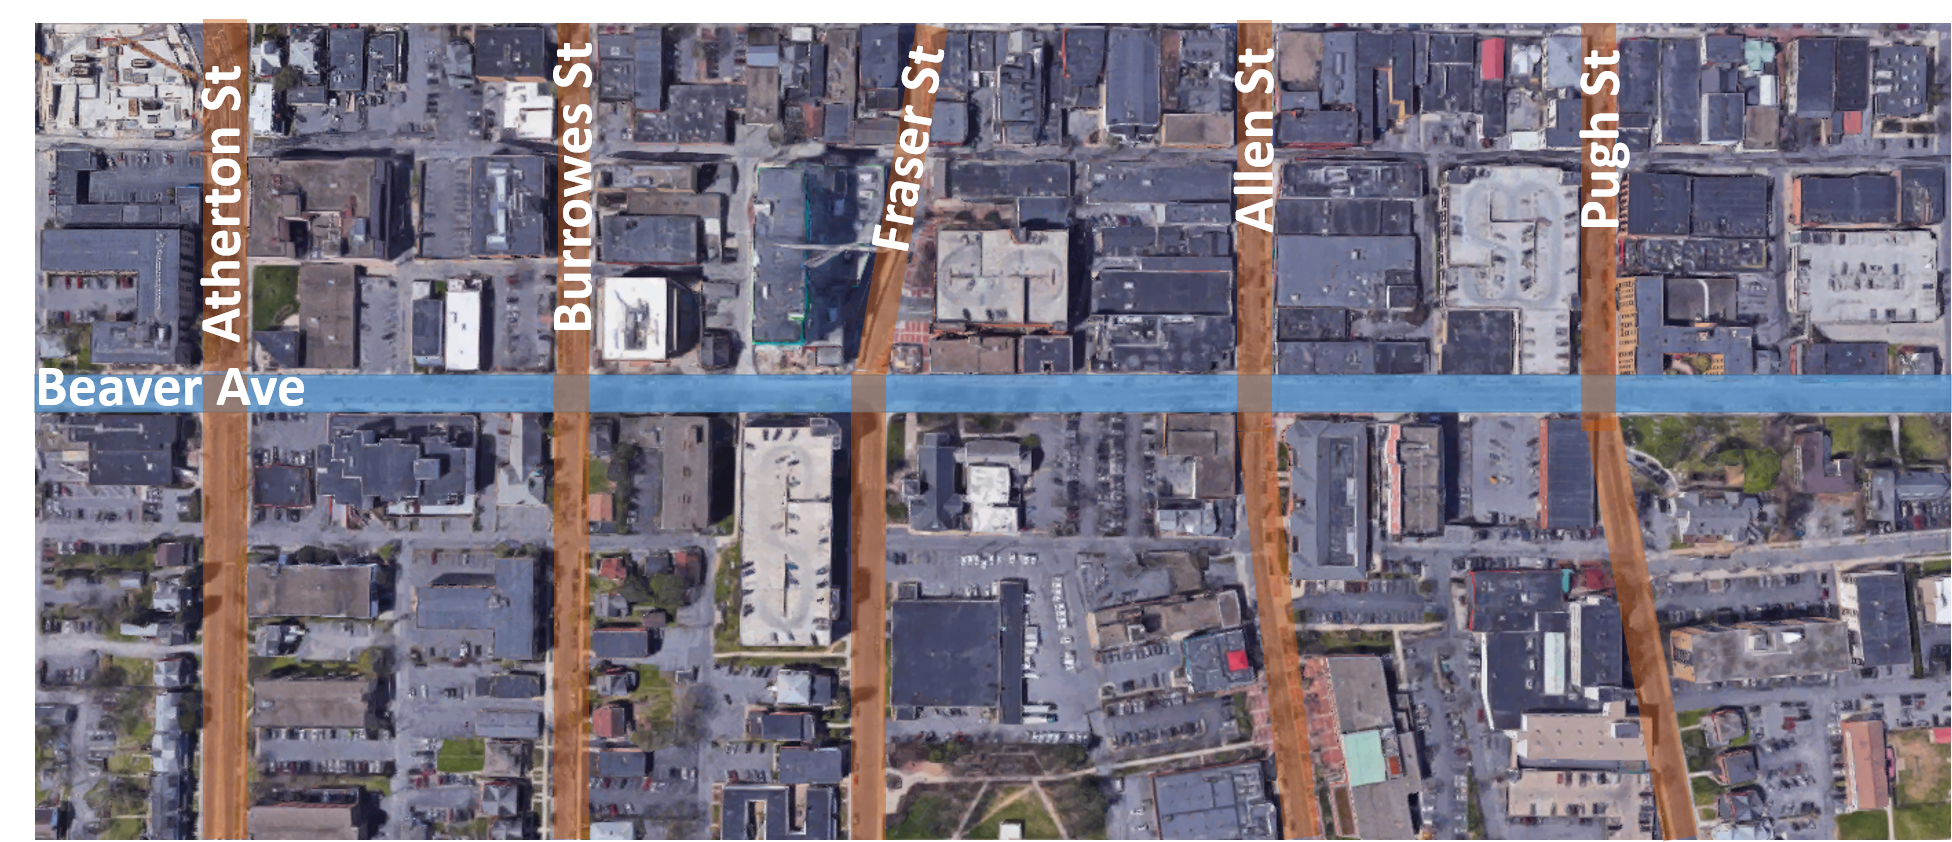
\includegraphics[width=0.8\textwidth]{figures/case_beaver.png}\\ 
    \begin{tabular}[c]{@{}c@{}}(a) Beaver Avenue in State College, Pennsylvania, USA: \\a 5-intersection arterial with unidirectional traffic on the arterial\\ and bidirectional traffic on the side streets.\end{tabular}\\
   \includegraphics[width=0.8\textwidth]{figures/case_intersection_note.png}\\
   \begin{tabular}[c]{@{}c@{}}(b) Qingdao Road in Jinan, China:\\ a 3-intersection arterial with bidirectional traffic \\on both the arterial and the side streets.\end{tabular}\\
%   \begin{tabular}[c]{@{}c@{}}(a) Beaver Avenue in State College, Pennsylvania, USA: \\a 5-intersection arterial with unidirectional traffic on the arterial\\ and bidirectional traffic on the side streets.\end{tabular}&
%   \begin{tabular}[c]{@{}c@{}}(b) Qingdao Road in Jinan, China:\\ a 3-intersection arterial with bidirectional traffic \\on both the arterial and the side streets.\end{tabular}\\
   \end{tabular}
   
     \caption{Real-world arterials for experiment.}
    \label{fig:real-intersection}
\end{figure*}

The free-flow speed on the road segments in above settings is set to 40 kilometers/hour. The traffic light in this part of experiment contains four phases: (1) WE-straight (green on WE straight going lane), (2) SN-straight (red on SN straight going lane), (3) WE-left (green on WE left turning lane), (4) SN-left (green on SN left turning lane) Every time the phase switches, a 5-second combined yellow and all-red time are followed to clear the intersection. Note that phase (3) and phase (4) would be disabled for when there is no turning traffic.
 
\subsubsection{Evaluation metric}
Following existing studies, we use the most frequently used measure, i.e., average travel time, to evaluate the performance (other measures show similar performance and are not shown here due to space limit):

\begin{itemize}
% \item \textbf{Queue length} ($Queue$) calculates average queue length over time, where the
% queue length at time $t$ is the sum of queue lengths over all approaching lanes. 
% \item  \textbf{Pressure} calculates the average pressure as defined above on each intersections at each time step. The pressure denotes the queuing stability inside the road network.
\item  \textbf{Travel time} calculates average travel time the vehicles spent on approaching lanes (in seconds). This is the most frequently used measure for traffic signal performance in transportation field.
\end{itemize}

% We also use \textbf{number of training rounds to converge} to measure the effectiveness of the training process of reinforcement learning agents.  

\subsubsection{Compared methods}
We compare our model with the following methods. It should be noted that all methods except the offsets of $\FT$ are carefully tuned and their best results are reported~\footnote{The codes including parameter settings is available at authors' website}. 

\begin{itemize}[wide,noitemsep,topsep=0pt]

\item \textbf{\FT}: Fixed-time with random offset~\cite{Roess2011t}. Each phase has fixed time of 15 seconds. For uni-directional traffic, there are only 2 phases (WE-straight, SN-straight). For traffic with turning vehicles, there are 4 phases. 

% The optimal cycle length of each intersection is calculated by close form solution as Equation~\ref{eq:cycle-length} given by the Webster's theory~\cite{Roess2011t}. The phase split percentage is equivalent with the percentage between the demand for a designated phase and total demand. The offsets are randomly selected to mimic an arterial with all traffic signals progressing independently. 

% \begin{equation}
% \label{eq:cycle-length}
% C_{min}=\frac{N\times{l}}{1-(\frac{v_c}{3600/h})}
% \end{equation}
% where $N$ is the number of phases in one cycle; $l$ is the lost time of a signal phase; $v_c$ is the maximum summation of volumes of critical lanes; $h$ headway of saturated traffic flow. 

\item \textbf{\Greenwave}: Green wave coordination on the arterial for unidirectional traffic~\cite{Roess2011t}. All intersections share the same cycle length, which is the maximum value of the cycle length for individual intersections calculated using Equation~\ref{eq:cycle-length}. The phase split percentage is equivalent with the percentage between the demand for a designated phase and total demand. Offsets between intersections are equivalent to the free-flow travel time between two consecutive intersections. %Vehicles traveling in the direction of green wave can benefit from a progressive cascade of green light without stopping at any intersections. 
\begin{equation}
\label{eq:cycle-length}
C_{min}=\frac{N\times{l}}{1-(\frac{v_c}{3600/h})}
\end{equation}
This is the most classical method in transportation field to implement coordination. However, \Greenwave is only an optimal solution for unidirectional and uniform traffic on the arterial. 

\item \textbf{\Maxpressure}: Max pressure control policy ~\cite{varaiya2013max}. \Maxpressure maximizes network throughput. The phase is determined by the pressure defined by the algorithm.

% optimal offsets to maximize the weighted combination of bandwidths for both directions of traffic along the arterial~\cite{little1981maxband}. The cycle length and phase split is calculated in the same  way as \Greenwave.

\item \textbf{\Deeplight} is an individual deep reinforcement learning approach proposed in \cite{wei2018intellilight}. This method does not consider context information.
%  \Deeplight is a single intersection control model that uses a representation of the local traffic information as state and reward function.

In addition to the baseline methods, we also consider several variations of our model.

\item \textbf{\SDeeplight}: By changing the state of \Deeplight from number of vehicles on each approaching lanes to the number of vehicles on each segment of lanes (coming vehicle distribution), with this more delicate state design, the agents will have more information than \Deeplight agents.

% \item \textbf{\SNDeeplight} The state is further modified as same as our proposed state, i.e., number of lane segments' vehicles on both approaching lanes and exiting lanes.

\item \textbf{\SNDeeplight} Our proposed method. 

Note that all the learning methods share the same neural network structure.


% \item \textbf{\NIPS} is a coordinated reinforcement learning approach for multi-intersection control~\cite{VaOl16}. Specifically, the coordination is achieved by designing a coordination graph and the joint local Q-function is defined on two intersections directly. Thus, this method can only optimize the joint action between two intersections.

\end{itemize}

% We denote our proposed method as \textbf{\PressLight}. We also compare a variation of our proposed method without network sharing, denoted as \textbf{\MDeeplight}.  

\subsection{Datasets}

\subsubsection{Synthetic data}

In the first part of the experiment, we use eight different configurations for synthetic traffic data, detailed in Table~\ref{tab:synthetic-table}. Note that all the traffic flow is uni-directed and there is no turning traffic. All the traffic is uniform, the demand in Table~\ref{tab:synthetic-table} is equal to critical lane volume ratios in the system, which is practically used to determine the phase split in field.

% Under each configuration, we have two variants on traffic: through traffic only (denoted as $\withoutturn$) and traffic with turns (20\% turning right and 20\% left, denoted as $\withturn$).Since all the traffic is uniform and evenly split among lanes, the demand in Table~\ref{tab:synthetic-table} is equal to critical lane volume ratios in the system, which is practically used to determine the phase split in field.

% \begin{table}[tbp!]
% \begin{center}
% \caption{Configurations for synthetic traffic data}
% \label{tab:synthetic-table}
% \begin{tabular}{c|c|c|c|c}
% \toprule
%  & \begin{tabular}[c]{@{}c@{}}Demand\\pattern \end{tabular}&\begin{tabular}[c]{@{}c@{}}
%   Arterial \\demand (cars/h)\end{tabular} &  \begin{tabular}[c]{@{}c@{}}Side-road\\ demand (cars/h) \end{tabular} &\begin{tabular}[c]{@{}c@{}}  Config\\ \#\end{tabular} \\ \hline
% %   \multicolumn{5}{*}{uniform}\\
% %   \hline
%  \multirow{4}{*}{Uniform} 
%  &\multirow{2}{*}{Unidirectional} & {300}    & 180   &1  \\ \cline{3-5} 
%                  &                & {700}    & 420   &2  \\\cline{2-5}
%  &\multirow{2}{*}{Bidirectional}  & {300}    & 180   &3  \\ \cline{3-5} 
%                   &               & {700}    & 300   &4  \\\bottomrule
%  \multirow{4}{*}{Dynamic} 
%  &\multirow{2}{*}{Flat} & {300}    & 180   &5  \\ \cline{3-5} 
%                   &               & {700}    & 420   &6  \\\cline{2-5}
%  &\multirow{2}{*}{Fluctuated}  & {300}    & 180   &7  \\ \cline{3-5} 
%                   &              & {700}    & 300   &8  \\\bottomrule
% \end{tabular}
% \end{center}
% \end{table}
\begin{table}[tbp!]
\begin{center}
\caption{Configurations for synthetic traffic data}
\label{tab:synthetic-table}
\begin{tabular}{c|c|c|c}
\toprule
  \begin{tabular}[c]{@{}c@{}}Demand\\pattern \end{tabular}&\begin{tabular}[c]{@{}c@{}}
  Arterial \\demand (cars/h)\end{tabular} &  \begin{tabular}[c]{@{}c@{}}Side-road\\ demand (cars/h) \end{tabular} &\begin{tabular}[c]{@{}c@{}}  Config\\ \#\end{tabular} \\ \hline
  % \multicolumn{5}{*}{uniform}\\
  % \hline
\multicolumn{4}{c}{Uniform}  \\
\hline
 \multirow{2}{*}{Unidirectional} & {300}    & 180   &1  \\      \cline{2-4} 
                                & {700}    & 420   &2  \\      \cline{1-4}
 \multirow{2}{*}{Bidirectional}  & {300}    & 180   &3  \\      \cline{2-4} 
                               & {700}    & 300   &4  \\      \bottomrule
\multicolumn{4}{c}{Dynamic}  \\
                 \hline
 \multirow{2}{*}{Flat} & {300}    & 180   &5  \\               \cline{2-4} 
                                & {700}    & 420   &6  \\     \cline{1-4}
 \multirow{2}{*}{Fluctuated}  & {300}    & 180   &7  \\        \cline{2-4} 
                                & {700}    & 300   &8 \\     \bottomrule
\end{tabular}
\end{center}
\end{table}

\paragraph{Traffic $\withoutturn$}
We test our method under through traffic $\withoutturn$ in the experiment for the following reasons: 

\begin{itemize}
\item Under this situation, we can verify whether the proposed technique has reached the optimal solution. In general, the problem of finding a globally optimal solution for agents with partial information is known to be intractable~\cite{bernstein2002complexity}. But under synthetic uniform unidirectional traffic without turning, the optimal solution is known ($\Greenwave$ on the arterial). So we only need to verify whether $\PressLight$ has reached the same state as $\Greenwave$ to know whether our method has converged to the optimal solution.
\item The through-only traffic do exist in real world, especially for arterials and highways. For example, the US Highway-1 near Monmouth Junction prohibits left-turn and always allows right-turn traffic.
\end{itemize}

\paragraph{Synthetic dynamic data to have the same statistical feature as real-world data in Jinan and Hangzhou, China} This dataset was synthesized after a statistical analysis of real-world traffic pattern in Jinan and Hangzhou. Specifically, we care the turning ratio, the maximum traffic volume and the ratio of arterial traffic flow and side-street flow most. This parameters are carefully chosen to imitate reality. As a result, all the vehicles on approaching lanes  will have 10\% of possibility to turn left and 30\% turning right. The maximum traffic volume is set to be 700 for over-saturated scenario and 300 for under-saturated scenario. The ratios of arterial traffic flow and side-street flow are chosen to be 0.3 and 0.6 respectively.

% \paragraph{Traffic $\withturn$}
% We also test our method under traffic with turns for a more general setting. All the vehicles on approaching lanes will have 20\% of possibility to turn left and 20\% turning right. For unidirectional settings, the traffic on side streets might only have left turns or right turns with 20\% of overall traffic.

\subsubsection{Real-world data}

% \subsubsection{Real-world data}
\paragraph{Traffic profile in State College, Pennsylvania, the United States} This traffic dataset was collected during a traffic signal re-timing project in State College, Pennsylvania, USA. Traffic movement counts were manually collected for each intersection in the downtown area for morning, midday and afternoon peak hours. The data were aggregated into hourly volumes for left turn, through and right turn movements. We use the traffic volumes of intersections on Beaver Avenue, an one-way arterial in downtown State College. Its aerial image is shown in Figure~\ref{fig:real-intersection}(a).

\begin{center}
\begin{table*}[]
\centering
\caption{Performance on synthetic data in the arterial with 6 intersections}
\label{tab:synthetic-result}
% Please add the following required packages to your document preamble:
% \usepackage{multirow}
% Please add the following required packages to your document preamble:
% \usepackage{multirow}
% Please add the following required packages to your document preamble:
% \usepackage{multirow}
\begin{tabular}{|c|c|c|c|c|c|c|c|c|}
\hline
Measure                  & \multicolumn{8}{c|}{Average travel time}                                        \\ \hline
\multirow{2}{*}{Config.} & \multicolumn{4}{c|}{Synthetic uniform} & \multicolumn{4}{c|}{Synthetic dynamic} \\ \cline{2-9} 
                         & 1       & 2        & 3       & 4       & 5       & 6        & 7       & 8       \\ \hline
\FT                          & 70.17        & 124.56   & 70.17   & 124.56  & 93.29   & 325.48   & 109.50  & 246.25  \\ \hline
\Greenwave                       & 62.36    & 75.88    & 65.31   & 79.93   & 98.39   & 263.36   & 124.09  & 286.85  \\ \hline
\Maxpressure                       & 63.29  & 161.60   & 66.39   & 147.88  & 74.30   & 262.26   & 82.37   & 225.60  \\ \hline
\Deeplight                      & 64.45     & 86.86    & 67.09   & 102.73  & 65.07   & 233.17   & 66.77   & 258.33  \\ \hline
\PressLight                     & 62.33     & 75.73    & 59.42   & 74.98   & 59.96   & 160.48   & 61.34   & 184.51  \\ \hline
\end{tabular}
\end{table*}
\end{center}

\begin{center}
\begin{table*}[tp!]
\centering
\caption{Comparison with variants of our methods}
\label{tab:variants-result}
\begin{tabular}{|c|c|c|c|c|c|c|c|c|}
\hline
\multicolumn{9}{|c|}{Variants of our methods}                                                                                                                                                                                     \\ \hline
Measure                      & \multicolumn{8}{|c|}{Average travel time}          \\ \hline
\multicolumn{1}{|c|}{Config} & \multicolumn{1}{c|}{1} & \multicolumn{1}{c|}{2} & \multicolumn{1}{c|}{3} & \multicolumn{1}{c|}{4} & \multicolumn{1}{c|}{5} & \multicolumn{1}{c|}{6} & \multicolumn{1}{c|}{7} & \multicolumn{1}{c|}{8} \\ \hline
\Deeplight     & 64.45                  & 86.86                  & 67.09                  & 102.73                 & 65.07                  & 233.17                 & 66.77                  & 258.33                 \\ \hline
\SDeeplight                   & 62.54                  & 81.03                  & 59.89                  & 92.26                  & 59.06                  & 207.98                 & 60.23                  & 191.86                 \\ \hline
\SNDeeplight     & 62.70 &	81.17	& 59.92	&95.86	&61.20	&200.28	&61.76	&196.34\\ \hline

IRL+n  & 62.84 &	83.63 &	61.49 &	90.68 &	67.32 &	201.56 &	68.47 &	281.21 \\ \hline

\PressLight    & 62.33                  & 81.19                  & 59.90                  & 84.71                  & 59.96                  & 160.48                 & 61.34                  & 184.51                 \\ \hline
\end{tabular}
\end{table*}
\end{center}

% % \begin{table}[]
% \begin{center}
% \begin{table*}[tp!]
% \caption{Performance on synthetic data in the arterial with homogeneous intersections}
% % \label{tab:synthetic-result}
% \begin{tabular}{|l|l|l|l|l|l|l|l|l|}
% \hline
% Measure & \multicolumn{4}{l|}{Average travel time} & \multicolumn{4}{l|}{Average pressure} \\ \hline
% Config. & 1        & 2       & 3        & 4        & 1       & 2       & 3       & 4       \\ \hline
% \multicolumn{9}{|c|}{3 INTERSECTIONS}                                                      \\ \hline
% FT      & 66.86    & 57.08   & 146.78   & 117.17   & 0.34    & 0.45    & 4.94    & 6.07    \\ \hline
% GW      & 62.80    & 53.71   & 67.50    & 65.28    & 0.18    & 0.28    & 0.87    & 2.01    \\ \hline
% MP      & 65.87    & 57.52   & 73.16    & 80.40    & 0.48    & 0.57    & 1.28    & 12.42   \\ \hline
% IRL     & 61.38    & 52.62   & 69.8     & 65.42    & 0.05    & 0.05    & 0.77    & 1.53    \\ \hline
% NIPS    &          &         &          &          &         &         &         &         \\ \hline
% NEW     & 60.48    & 52.5    & 66.43    & 65.56    & 0.05    & 0.05    & 0.43    & 1.42    \\ \hline
% \multicolumn{9}{|c|}{10 INTERSECTIONS}                                                     \\ \hline
% FT      & 111.31   & 78.78   & 180.78   & 129.20   & 0.24    & 0.29    & 1.87    & 2.94    \\ \hline
% GW      & 95.74    & 69.64   & 100.68   & 80.74    & 0.15    & 0.24    & 0.71    & 1.67    \\ \hline
% MP      & 95.37    & 73.44   & 112.39   & 128.92   & 0.29    & 0.49    & 1.42    & 4.57    \\ \hline
% IRL     & 93.78    & 66.86   & 110.14   & 91.01    & 0.05    & 0.02    & 0.96    & 2.18    \\ \hline
% NIPS    &          &         &          &          &         &         &         &         \\ \hline
% NEW     & 91.52    & 67.45   & 92.26    & 103.44   & 0.06    & 0.07    & 0.76    & 2.35    \\ \hline
% \end{tabular}
% \label{tab:result_syn}
% \end{table*}
% \end{center}

% \begin{center}
% \begin{table*}[tp!]
% \caption{Performance on synthetic data in the arterial with homogeneous intersections}
% \label{tab:synthetic-result}
% \centering
% \begin{tabular}
% {p{0.05\textwidth}p{0.03\textwidth}p{0.03\textwidth}p{0.03\textwidth}p{0.03\textwidth}p{0.03\textwidth}p{0.03\textwidth}p{0.03\textwidth}p{0.03\textwidth}|p{0.035\textwidth}p{0.035\textwidth}p{0.035\textwidth}p{0.035\textwidth}p{0.035\textwidth}p{0.035\textwidth}p{0.035\textwidth}p{0.035\textwidth}}
% \toprule
% Measure & \multicolumn{8}{c|}{$Queue$}& \multicolumn{8}{|c}{$Time$} \\
% \hline
% Config. & 1     & 2     & 3     & 4     & 5    & 6      & 7     & \multicolumn{1}{c|}{8}     & 1      & 2     & 3      & 4      & 5      & 6      & 7      & 8      \\
% \hline
% \multicolumn{17}{c}{2-intersection arterial under traffic $\withoutturn$ (through traffic only)}                                                                                                                                               \\
% \hline
% \FT      & 0.62  & 0.91  & 2.09   & 3.07  & 1.26 & 1.83   & 4.20   & \multicolumn{1}{c|}{6.24}  & 52.65  & 49.17 & 62.86  & 58.43  & 52.65  & 49.17  & 62.85  & 58.43  \\
% \Greenwave      & 0.59  & 0.99  & 1.31  & \textbf{2.3}   & 1.19 & 1.98   & 4.25  & \multicolumn{1}{c|}{6.24}  & 51.77  & 49.01    & \textbf{51.92}  & \textbf{52.29}  & 51.79  & 49.01  & 60.27  & 56.53  \\
% \Max & -     & -     & -     & -     & 1.89 & 1.69   & 2.21  & \multicolumn{1}{c|}{\textbf{5.72}}  & -      & -     & -      & -      & 57.36  & 47.81  & 53.88  & 56.57  \\
% \Deeplight     & 0.70   & 0.70   & 1.28  & 4.81  & 1.55 & 1.61   & 2.60   & \multicolumn{1}{c|}{7.86}  & 54.53  & 47.43 & 53.01  & 63.57  & 53.79   & 47.24  & 52.05  & 58.75  \\
% \NIPS    & 0.56  & 0.80   & 1.59  & 2.77  & \textbf{0.73} & 1.79 & 21.65 & \multicolumn{1}{c|}{10.00}    & 51.31  & 47.5  & 52.06  & 52.55  & 50.33  & 54.42  & 272.76 & 67.46  \\
% \PressLight    & \textbf{0.41}  & \textbf{0.54}  & \textbf{1.00}     & 2.80   & 0.83 & \textbf{0.92}   & \textbf{1.95}  & \multicolumn{1}{c|}{6.23}  & \textbf{50.03}  & \textbf{45.73} & 52.13  & 53.83  & \textbf{50.11}  & \textbf{45.52}  & \textbf{51.94}  & \textbf{56.18}  \\
% \hline
% \multicolumn{17}{c}{3-intersection arterial under traffic $\withoutturn$ (through traffic only)}                                                                                                                                               \\
% \hline
% \FT      & 0.98  & 0.52  & 2.12  & 3.09  & 1.96 & 1.04   & 4.23  & \multicolumn{1}{c|}{6.27}   & 65.91  & 57.5  & 79.96  & 69.3   & 65.9   & 57.53  & 79.93  & 69.32  \\
% \Greenwave      & 0.53  & 0.92  & 1.15  & \textbf{2.1}   & 1.06 & 1.85   & 4.5   & \multicolumn{1}{c|}{6.42}  & 63.85  & 56.73 & \textbf{63.86}  & \textbf{60.02}  & 63.86  & 56.71  & 76.49  & 66.77  \\
% \Maxband & -     & -     & -     & -     & 1.54 & 2.09   & \textbf{2.00}  & \multicolumn{1}{c|}{\textbf{5.48}}  & -      & -     & -      & -      & 67.45  & 57.87  & 67.52  & \textbf{64.37}  \\
% \Deeplight     & 0.8   & 0.55  & 1.55  & 4.13  & 1.05 & 1.16   & 2.72  & \multicolumn{1}{c|}{9.28}  & 67.41  & 52.90  & 67.56  & 69.48  & 63.31  & 53.52  & 66.52  & 70.38  \\
% \NIPS    & 0.563 & 0.346 & 2.88  & 2.92 & 1.19 & 1.39   & 3.77  & \multicolumn{1}{c|}{26.11} & 64.45  & 53.02 & 80.05  & 142.09 & 63.79  & 53.94  & 69.29  & 109.49 \\
% \PressLight    & \textbf{0.35}  & \textbf{0.43}  & \textbf{0.89}  & 2.36  & \textbf{0.72} & \textbf{0.76}   & 2.03  & \multicolumn{1}{c|}{6.22}  & \textbf{61.94}  & \textbf{52.54} & 64.08  & 62.17  & \textbf{62.50}   & \textbf{52.33}  & \textbf{65.06}  & 65.27  \\
% \hline
% \multicolumn{17}{c}{4-intersection arterial under traffic $\withoutturn$ (through traffic only)}                                                                                                                                               \\
% \hline
% \FT      & 0.56  & 0.87  & 2.13  & 3.11  & 1.12 & 1.75   & 4.25  & \multicolumn{1}{c|}{6.81}   & 75.04  & 62.61 & 92.31  & 76.31  & 75.04  & 62.62  & 92.31  & 76.31  \\
% \Greenwave      & 0.5   & 0.94  & 1.06  & \textbf{2.17}  & 1.01 & 1.88   & 4.53  & \multicolumn{1}{c|}{6.9}   & 72.75  & 61.78 & \textbf{72.71}  & \textbf{66.07}  & 72.76  & 61.79  & 87.79  & 74.42  \\
% \Maxband & -     & -     & -     & -     & 1.79 & 2.38   & 1.84  & \multicolumn{1}{c|}{\textbf{5.66}}  & -      & -     & -      & -      & 79.44  & 64.91  & 76.39  & 72.66  \\
% \Deeplight     & 0.6   & 0.58  & 1.63  & 9.51  & 0.79 & 0.92   & 3.3   & \multicolumn{1}{c|}{9.62}  & 75.57  & 58.83 & 80.42  & 190.5  & 70.74  & 57.18  & 78.02  & 78.54  \\
% \NIPS    & 0.54  & 0.60   & 1.28  & 5.99  & 0.56 & 1.18   & 8.59  & \multicolumn{1}{c|}{29.86} & 72.94  & 59.44 & 91.23  & 77.75  & 69.95  & 56.74  & 95.21  & 197.8  \\
% \PressLight    & \textbf{0.32}  & \textbf{0.40}   & \textbf{0.87}  & 2.47  & \textbf{0.50}  & \textbf{0.70}    & \textbf{1.61}  & \multicolumn{1}{c|}{6.53}  & \textbf{70.68}  & \textbf{56.92} & 73.23  & 67.13  & \textbf{70.37}  & \textbf{56.67}  & \textbf{73.07}  & \textbf{72.30}   \\
% \hline
% \multicolumn{17}{c}{10-intersection arterial under traffic $\withoutturn$ (through traffic only)}                                                                                                                                               \\
% \hline
% \FT      & 1.24  & 1.71  & 2.12  & 3.10  & 2.65 & 3.57   & 4.22  & \multicolumn{1}{c|}{6.16}  & 131.51 & 96.23 & 136.36 & 101.21 & 131.88 & 96.45  & 136.61 & 101.33 \\
% \Greenwave      & 0.36  & 0.60  & 0.79  & \textbf{1.61}  & 1.28 & 2.19   & \textbf{1.48}  & \multicolumn{1}{c|}{\textbf{3.40}}  & 103.24 & 76.62 & 105.98 & 81.65  & 112.46 & 84.22  & 103.88 & 86.53  \\
% \Maxband & -     & -     & -     & -     & 1.91 & 2.48   & 1.67  & \multicolumn{1}{c|}{4.96}  & -      & -     & -      & -      & 108.89 & 78.73  & 103.32 & 84.11  \\
% \Deeplight     & 0.65  & 0.47  & 1.71  & 3.55  & 0.57 & 0.79   & 2.31  & \multicolumn{1}{c|}{7.60}  & 93.90  & 72.41 & 108.27 & 97.08  & 87.96  & 72.12  & 96.73  & 97.70  \\
% \NIPS    & 0.67  & 3.47  & 16.04 & 17.00 & 1.33 & 2.52   & 24.65 & \multicolumn{1}{c|}{31.91} & 109.53 & 82.59 & 248.72 & 263.04 & 109.85 & 144.72 & 212.51 & 206.55 \\
% \PressLight    & \textbf{0.34}  & \textbf{0.29}  & \textbf{0.75}  & 1.86  & \textbf{0.47} &  \textbf{0.65}  &  1.54 & \multicolumn{1}{c|}{4.43}      & \textbf{88.56}  & \textbf{70.45} & \textbf{88.56}  & \textbf{80.27}  &    \textbf{40.66} &   \textbf{70.78}  & \textbf{90.74}  & \textbf{83.41} \\ 

% \hline
% \multicolumn{17}{c}{4-intersection arterial under traffic $\withturn$ (with left and right turn traffic)}                                                                                                                                               \\
% \hline
% \FT      & 1.07 & 1.52 & 1.63 & 2.47 & 2.16 & 3.18   & 5.27 & 4.55 & 76.68 & 70.02 & 76.97 & 71.37 & 77.51 & 71.54 & 91.93 & 85.41 \\
% \Greenwave      & 0.49 & 0.85 & 0.81 & 1.81 & 1.24 & 2.20   & 1.55 & 2.27 & 67.26 & 62.77 & 67.20 & 65.51 & 67.26 & 62.97 & 67.20 & 65.51 \\
% \Maxband & -    & -    & -    & -    & 1.43 & 2.09   & 1.73 & 3.71 & -     & -     & -     & -     & 71.20 & 71.74 & 65.93 & 77.75 \\
% \Deeplight     & 0.33 & 0.69 & 0.67 & 1.13 & 0.66 & 1.6    & 1.3  & 1.31 & 64.99 & 61.68 & 66.67 & 62.41 & 65.28 & 63.02 & 68.68 & 67.43 \\
% \NIPS    & 0.33 & 0.67 & 0.88 & 1.05 & 0.86 & 228.00 & 5.08 & 1.99 & 65.69 & 61.98 & 68.43 & 62.82 & 67.59 & 75.50 & 84.87 & 69.01 \\
% \PressLight    & \textbf{0.28} & \textbf{0.63} & \textbf{0.56} & \textbf{1.00} & \textbf{0.53} & \textbf{1.44}   & \textbf{1.05} & \textbf{1.03} & \textbf{64.60} & \textbf{61.56} & \textbf{66.24} & \textbf{62.29} & \textbf{64.78} & \textbf{62.85} & \textbf{65.34} & \textbf{66.81} \\

% \bottomrule
% \end{tabular}
% \label{tab:result_syn}
% \end{table*}
% \end{center}


\paragraph{Surveillance camera data in Jinan, China}
The real-world dataset are collected by road-side surveillance cameras in Jinan, China over the time period from 08/01/2016 to 08/31/2016. In every second, the camera gathers records about the vehicles passing though the camera consisting time, camera ID, direction and vehicle plate ID. By analyzing these records with camera locations, the trajectories of vehicles are recorded.
We use the time of vehicles entering these intersections as traffic flow for experiments. We feed this real-world traffic into SUMO as on-line experiments. We select an arterial with 3 intersections, as shown in Figure~\ref{fig:real-intersection}(b). The reason we select this case is because all these 3 intersections have 4-way surveillance cameras that describe the comprehensive view of the traffic conditions.

\subsection{Performance on synthetic data}

\subsubsection{Comparison with state-of-the-art methods} 


% \begin{figure}[htb]
%   \centering
% 	\includegraphics[width=0.48\textwidth]{figures/offset_draft.pdf}
%      \caption{Bidirectional traffic on an arterial with 6 intersections.}   
%     \label{fig:case-study}
% \end{figure}

% \begin{figure*}[thb]
%   \centering
%   \begin{tabular}{cc}
%   \includegraphics[width=0.42\textwidth]{figures/offset_draft.pdf} &
% %   \includegraphics[width=0.45\textwidth]{figures/case_study_2_bi.png} \\
%   \begin{tabular}[c]{@{}c@{}}(a) Synthetic data configuration 1 on a 4-intersection arterial\end{tabular}&
% %   \begin{tabular}[c]{@{}c@{}}(b) Synthetic data configuration 5 on a 2-intersection arterial\end{tabular}\\
%   \end{tabular}
% \caption{Space-time diagrams with signal timing plans to illustrate the learned unidirectional (a) and bidirectional (b) green waves from synthetic data. The green-yellow-red bands represent the learned signal plans on \WE. Each line in space-time diagram stands for one vehicle's trajectory. The trajectory of a vehicle in the green wave will be a straight sloped line in the space-time diagram.}
%     \label{fig:case-study}
% \end{figure*}

We first compare our method with four other baselines under 8 configurations on an arterial with 6 intersections. From Table~\ref{tab:synthetic-result}, we can see that: 
% Note that \Maxband only works when there is bidirectional traffic. From Table~\ref{tab:synthetic-result}, we can see that: 

1) Our proposed method \PressLight can achieve the best performance for most of the settings compared with state-of-the-arts. \Greenwave is designed for unidirectional uniform traffic. Hence, under configuration 1 and 2, \Greenwave achieves best travel time. Our proposed method could achieve similar performance. This demonstrates that,even without explicit coordination, our RL agents can learn the coordination implicitly. For bidirectional or dynamic traffic (configuration 3-8), \Maxpressure is more capable. However, as a rule based control, the inherit parameters within \Maxpressure is hard to tune, thus emphasizing the effectiveness of our learning based agents. \Deeplight also achieves good performance for all of the settings and our method is always better, which verifies the effectiveness of our proposed state and reward design.

% Some baselines perform well on certain setting (e.g., \Greenwave achieves good travel time under configuration 1 and 2 and \Maxpressure is more capable dealing with bi-directional traffic (configuration 3-8), our proposed methods could always achieve similar or better performances. This also demonstrates that,even without explicit coordination, our RL agents can learn the coordination implicitly. Compared with individual control (\IRL), it is shown that coordination could be learned with our new design of sate and reward of RL agents. 

% including the method with explicit coordination strategies (\Greenwave) \nop{ \Maxband and \NIPS}, as is shown in Table~\ref{tab:synthetic-result}. This demonstrates that, even without explicit coordination, our RL agents can learn the coordination implicitly. Although some baselines perform well on certain setting (e.g., \Greenwave achieves good travel time under configuration 1 and 2, while our method also achieves similar performances), they perform badly in other configurations. This is because those methods are designed for these settings, e.g., \Greenwave is designed for unidirectional uniform traffic, \Maxband is designed for bidirectional uniform traffic, and \NIPS is designed for two-intersection regional control.
% {\color{blue}maxpressure is better than greenwave for bidirectional traffic}

2) For dynamic traffic, which is a more realistic, our method always achieves the best performance. In Table~\ref{tab:synthetic-result}, for configuration 5-8, our method steadily outperform all other baselines in terms of travel time. Is shows that learning agents is able to adapt to changing traffic. 

3)When the traffic volume grows to larger (configuration 4, 6 and 8), our method becomes much better than other baselines. This is because our agents, inspired by \Maxpressure, consider to balance the traffic pressure on all of the intersections with the road network.

In summary, our method \PressLight shows better performance under different configurations.

% When there is turning traffic $\withturn$, which is a more realistic setting, our method also outperform other methods. This is mainly because \Greenwave and \Maxband only consider the traffic that travels along the arterial, and \NIPS only optimizes the joint action for two intersections. In summary, our method \PressLight shows better performance under different configurations.

% \subsection{Performance on dynamic data}

\subsubsection{Comparison with variants of our proposed method}  
We compare several variation of our method to validate the effectiveness of state and reward design. Table~\ref{tab:variants-result} shows the performance of variants of our proposed method. First we can see that by adding context information, it immediately boost the performance of individual control agents for all settings. It is able to achieve similar best performance under unidirectional and traffic with small flow (configuration 1, 2, 3, 5 and 6). However, for over-saturated bidirectional traffic scenario, optimizing queue length of each agents individually would ignore the congestion on neighboring intersections. Hence, inspired by \Maxpressure, the reward is modified from minimizing queue length to minimizing the difference of queue lengths of all the approaching lanes and queue lengths of exiting lanes. To make sure that the agent is able to observe traffic distribution on exiting lanes, vehicle distribution on exiting lanes are added into state design. It turns out that by balancing the queues for each intersection, it further boost the performance under over-saturated traffic. In addition, another variants, \SNDeeplight, with same state but no modification on reward is investigated too. The result shows that given more state information would not significantly boost the performance, but somehow interfere the convergence speed thus resulting in no improvement compared to \SDeeplight.

% to optimize pressure, by which the queue 
% without information of exiting approaches, the agents may fail
% But it does not achieve best when the traffic volumes grow larger.

% \Todo{state that reward and state information is necessary}
% 3>2>1>0
% We compare a variation of our method to validate the effectiveness of sharing the network.
% Results in Table~\ref{tab:entropy} show that \PressLight shows a better stability than \MDeeplight under both homogeneous and heterogeneous situations. This is because the network parameters are shared transferred from a similar intersection agent model serves as a good guidance to help the model converge faster as well as build up its robustness. For arterials with heterogeneous intersections, the values of entropy of all settings for both \MDeeplight and \PressLight are higher than those in homogeneous settings, indicating the structure of network does affects the convergence of RL agents.


\subsubsection{Our proposed reward - pressure is correlated with travel time}  
To show the correlation of our proposed reward--pressure and average travel time, we draw a figure to show the process of convergence by plotting the average reward (pressure) each round with average travel time each round. Figure~\ref{fig:convergence} illustrates the correlation between pressure and travel time.

% \Todo{justifying reward figure -- convergence figure}

\begin{figure}[t!]
\centering
  \begin{tabular}{c}
   \includegraphics[width=0.8\textwidth]{figures/converg.pdf} \\
   \end{tabular}
     \caption{Correlation of average duration and pressure.}
    \label{fig:convergence}
\end{figure}



% \Todo{if we have time}
\subsubsection{Number of intersections}
% \Todo{table here}
We employ our model where we vary the number of intersections from 6 to 10. Table~\ref{tab:number_of_intersections} illustrates the performance of configuration 1-4 for our model and \Maxpressure. The conclusion could be drawn that our model could achieve better performance even when the number of intersections grows.

\begin{table}[]
\centering
\caption{Performance in a 10-intersection arterial}
\label{tab:number_of_intersections}
\begin{tabular}{|c|c|c|c|c|}
\hline
Measure & \multicolumn{4}{c|}{Average travel time} \\ \hline
Config. & 1        & 2        & 3       & 4        \\ \hline
\Maxpressure      & 68.78    & 129.63   & 68.78   & 129.63   \\ \hline
\textbf{\PressLight}    &      \textbf{66.27}    &     \textbf{88.88}     & \textbf{67.18}   & \textbf{79.61}    \\ \hline
\end{tabular}
\end{table}


\begin{table}[]
\centering
\caption{Performance on real-world data}             
\begin{tabular}{|c|c|c|}
\hline
Config                             & Beaver               & Jinan          \\ \hline
Measure                            & Travel time          & Travel time    \\ \hline
\FT                                 & 336.29          & 317.40    \\ \hline
\Greenwave                                 & 332.06          & 370.30    \\ \hline
\Maxpressure                                 & 222.90          & 567.06    \\ \hline
\Deeplight                                & 338.52          & 58.18          \\ \hline
% \multicolumn{3}{|c|}{Variants of our methods}                              \\ \hline
% \SDeeplight                         & 151.70          & 56.12          \\ \hline
\textbf{\PressLight} & \textbf{92.00} & \textbf{54.87} \\ \hline
\end{tabular}
\label{tab:real_result}
\end{table}

% \begin{table}[t!]
% \centering
% \caption{Performance on real-world data}
% \begin{tabular}
% {p{0.06\textwidth}p{0.06\textwidth}p{0.08\textwidth}p{0.001\textwidth}p{0.06\textwidth}p{0.06\textwidth}}
% \toprule
%         & \multicolumn{2}{c}{\begin{tabular}[c]{@{}c@{}}Beaver  Avenue\\ in State College\end{tabular}} & & \multicolumn{2}{c}{\begin{tabular}[c]{@{}c@{}}Qingdao Road\\ in Jinan\end{tabular}} \\ \hline
%         & $Queue$   & \multicolumn{1}{l|}{$Time$\ \ \ } & & $Queue$   & $Time$ \\ \hline
% \FT      & 1.83    &  \multicolumn{1}{l|}{58.63} & & 7.85  & 159.20 \\
% \Greenwave & 1.24   &  \multicolumn{1}{l|}{48.56}& & 5.73  & 140.71  \\
% \Deeplight     & 0.7 &  \multicolumn{1}{l|}{38.29}&  & 2.80   & 95.86  \\
% \Maxband & -      &  \multicolumn{1}{l|}{- }&        & 1.84   & 97.97  \\
% \NIPS    & 1.83   &  \multicolumn{1}{l|}{37.28}&     & 1.39   & 97.66  \\  \hline
% \MDeeplight     &  0.62 & \multicolumn{1}{l|}{37.01}&  & 1.75 & 89.23  \\
% \PressLight     & \textbf{0.27}  &  \multicolumn{1}{l|}{\textbf{36.30}}&  & \textbf{1.34} & \textbf{86.25}  \\   
% \bottomrule
% \end{tabular}
% \label{tab:real_result}
% \end{table}


\subsubsection{Green wave learned from RL agents}

\begin{figure}[htb]
  \centering
	\includegraphics[width=0.8\textwidth]{figures/offset.pdf}
     \caption{Offsets between intersections learnt by RL agents}   
    \label{fig:case-study}
\end{figure}

To validate that our method can learn an optimal solution under ideal conditions (configuration 2), we use the synthetic setting where conventional coordination method \Greenwave can form a green wave for traffic along the arterial and is an optimal solution as stated in ~\cite{Roess2011t}. The \Greenwave offset $\Delta$ equals to the block length $l$ between two consecutive intersections divided by free-flow speed $v$, and the optimal phase split is equal to the percentage between the demand for a designated phase and total demand. In our experiments, $l\approx 300$ m, $v\approx 10$ m/s, hence, the optimal offset should be $\Delta\approx 30$ s, and the optimal phase split should be 1:0.6 (Green-\WE : Red-\WE). However, the min action time of our agents is 10s, hence the result of the control policy learned does not fit into the theoretically calculated optimal solution. Specifically, we use time-space diagrams to show trajectories of vehicles and phase plans of traffic signal controllers, as it is shown in Figure~\ref{fig:case-study}. 

\begin{figure*}[t!]
  \centering
  \begin{tabular}{c}
   \includegraphics[width=0.85\textwidth]{figures/case_study_real_1.png} \\
   \end{tabular}
     \caption{Space-time diagram with signal timing plan to illustrate the learned coordination strategy from real-world data on the arterial of Qingdao Road in the morning (around 8:30 a.m.) of August 6th.}
    \label{fig:case-study-real}
\end{figure*}

A time-space diagram is drawn with time on the horizontal axis and distance (from a reference point, here we use the westernmost point on the arterial as the reference point) on the vertical axis, exampled as Figure~\ref{fig:case-study} and~\ref{fig:case-study-real}. A learned offset was visualized in the diagram. Vehicles move across 6 traffic lights with distance from 0 to 1800. Hence, the dotted line in the Figure~\ref{fig:case-study} could be seen as a possible vehicle trajectory. The slope indicates free flow speed. Traffic signal offset is indicated and it is approximately 25s or 30s between every 2 traffic signals.

% Vehicle trajectories are plotted on the time-space diagram and the difference in distance over time (distance divided by time, or change in $y$ divided by $x$) represents the speed or a sloped line on the diagram. The trajectories for vehicles on the arterial always move left to right along with time, and as shown the distance traversed can be either eastbound (bottom to top of the diagram) or westbound (top to bottom). Vehicles can have a positive or negative slope that indicates the movements on the street network. Stopped vehicles (no change in distance) are shown as horizontal lines. Vehicles traversing green waves (always at their free-flow speed) will be straight sloped lines.


% Vehicle trajectories are plotted on the time-space diagram and the difference in distance over time (distance divided by time, or change in $y$ divided by $x$) represents the speed or a sloped line on the diagram. The trajectories for vehicles on the arterial always move left to right along with time, and as shown the distance traversed can be either eastbound (bottom to top of the diagram) or westbound (top to bottom). Vehicles can have a positive or negative slope that indicates the movements on the street network. Stopped vehicles (no change in distance) are shown as horizontal lines. Vehicles traversing green waves (always at their free-flow speed) will be straight sloped lines.


For unidirectional traffic, as is shown in Figure~\ref{fig:case-study}(a), our method not only forms a green wave for vehicles on the arterial, but also learns the optimal cycle length and phase split, which is 50s and 1:0.6 (Green-\WE:25s Red-\WE:15s Yellow-phase:5+5). 

% For bidirectional traffic, while it is hard to form a green wave because it has strict requirements on the road structures (i.e., the blocks along the arterial to be identical) and on the relationships between cycle length and free-flow speed, our method can also learn the bidirectional {\Greenwave} with zero offsets and the optimal cycle length equals to the free-flow travel time between consecutive intersections, as is shown in Figure~\ref{fig:case-study}(b). This experiment further proves the capability of out RL model to learn bidirectional {\Greenwave} signal settings without any prior knowledge, providing maximum green bandwidth for both directions ~\cite{Roess2011t}.


\subsection{Performance on real-world data}
\subsubsection{Comparison of different methods} In this section, we compare our method with baseline methods on real-world data. The overall results are shown in Table~\ref{tab:real_result}.
From Table~\ref{tab:real_result}, we can see that our method \PressLight achieves the best result over all the compared methods in terms of queue length and travel time, with a relative improvement of 61\% and
3\% in the setting of Beaver Avenue, and 4\% and 12\% in the setting of Qingdao Road correspondingly over the best baseline method.
% In addition, \PressLight outperforms \MDeeplight steadily, indicating the effectiveness of transferred knowledge.


\subsubsection{Green wave learned from RL agents}
In this section,
we make observations on the policies we learned from the real
data for the arterial of Qingdao Road (\WE and \EW ) at Lashanhedong Road (\SN-1 and \NS-1), Zibo Road (\SN-2 and \NS-2) and Dongying Road (\SN-3 and \NS-3) during the morning peak hour (around 8:30 a.m.) on August 6th. 


A time-space diagram is drawn with time on the horizontal axis and distance (from a reference point, here we use the westernmost point on the arterial as the reference point) on the vertical axis, exampled as Figure~\ref{fig:case-study-real}. 

Vehicle trajectories are plotted on the time-space diagram and the difference in distance over time (distance divided by time, or change in $y$ divided by $x$) represents the speed or a sloped line on the diagram. The trajectories for vehicles on the arterial always move left to right along with time, and as shown the distance traversed can be either eastbound (bottom to top of the diagram) or westbound (top to bottom). Vehicles can have a positive or negative slope that indicates the movements on the street network. Stopped vehicles (no change in distance) are shown as horizontal lines. Vehicles traversing green waves (always at their free-flow speed) will be straight sloped lines.

In Figure~\ref{fig:case-study-real}, most of the blue and orange lines are straight, indicating most vehicles on main road (including both \WE and \EW direction), are not stopped by red lights. This indicates that our method can automatically form a green wave under the real-world traffic.


% !TEX root = main.tex
\section{Conclusion}
In this chapter, we propose a novel RL method for multi-intersection traffic signal control on the arterials. We conduct extensive experiments using both synthetic and real-world experiments and demonstrate the superior performance of our method over state-of-the-art methods. Specifically, we draw a connection between reinforcement learning with conventional transportation control methods. It is the first time there exists a RL model automatically achieving coordination along a arterial without explicit priori knowledge. 
 
 We also acknowledge the limitations of our current approach and possible future directions could be the following. First, we can extend the tested corridor with more intersections, which will involve more complicated yet more realistic settings. The authors would expect increased computational cost while introducing more agents, however, our RL model is still elegant as there is no need for further model modifications. Secondly, our model is currently tested on a simulation environment, thus the feedbacks of control is also simulated. A field study is needed to validate our method in the real-world environment. Lastly, since the real-world traffic condition is a compound of cars, motorcycles, bikes and pedestrians, a comprehensive coordination between different parties should also be investigated. 